\chapter{Introduction}
\label{chap:intro}

Malicious software (malware), has long been a burden on users of computers and the internet. 
For individuals, a malware attack can cause the loss of their personal data and may allow hackers to access their bank accounts, steal their identity, or hold all of the files on their computer ransom. 
For a business, the effects can be extremely dire, with the average cost of a malware attack sitting around \$1.7 million~\cite{seals2019threatlist}. 
This problem is continuing to grow, and malware authors innovate in an effort to circumvent existing mitigating controls. 
As the IRA said to Margaret Thatcher after the Brighton Hotel Bombing: ``We only have to be lucky once. You will have to be lucky always''~\cite{thomas1984this}. 
So too is the case for malware, which must only find one vulnerable system to cause immense damage, while defenders must be lucky on all of their systems. 
As such, traditional signature-based antivirus engines have become less effective against unseen strains of malware~\cite{oconnor2017how}, and so machine learning techniques have helped provide detection of these threats on the endpoint.

In the case of mobile malware, we often do not have the luxury of running computationally intensive processes on an endpoint, nor do we have the ability to control devices which we do not own that are brought into our environment. 
As such, we need to leverage this same machine learning technology to perform endpoint-agnostic network detection of malware threats. 
In these cases, a network-based solution seems ideal, as this allows us to mitigate vectors commonly used by modern worms~\cite{mohurle2017brief}. 
Traditional intrusion detection systems like Snort continue to mitigate known threats, but these signature-based systems suffer from the same curse of reactivity as the traditional antivirus. 
In order to mitigate these threats, mitigating controls must be learned on the fly instead of reactively post-hoc by a human analyst.

Machine learning is a form of statistical learning which emphasizes predictions and pattern recognition in data~\cite{james14introduction}.
Generally, machine learning is viewed as a subset of artificial intelligence where algorithms build mathematical models based on sample data in order to make predictions without being programmed to do so~\cite{bishop2006pattern}.
Machine learning is broadly divided into 3 categories: 
Supervised learning, where a function to map data to a set of associated labels is learned;
Unsupervised learning, where groupings or clusters of the data are identified without labels;
and Reinforcement learning, which is concerned with experiential learning through agent interactions with an environment.
Though there are more granular categories, these suffice for most purposes.
In our case, we are concerned with a classification task for data where we do have labels - so we concern ourselves with supervised learning throughout this work. 


\section{Neural Networks}\label{intro:nn}
Neural Networks are a type of connectionist machine learning system in which artificial neurons are connected to one another in an attempt to emulate biological cognitive functions.
Each neuron is a node which connects to others in a way that mimics the dendrite-synapse-axon connections, illustrated in \ref{fig:neuron}.
Each of these links, similar to the myelin sheat in the brain, has a weight that determines the strength of any node on another.

Deep learning~\cite{goodfellow2016deep} is a particular form of machine learning in which artificial neurons are stacked on top of one another in two or more layers. 
Having a larger number of layers allows the network to learn increasingly complex representations at the cost of training speed and the need for more data. 
This has reasonably led us to ask what the applicability of neural networks and deep learning are to domains other than natural language processing~\cite{goldberg2016primer} and computer vision~\cite{lecun1998gradient}.

\begin{figure}\label{fig:neuron}
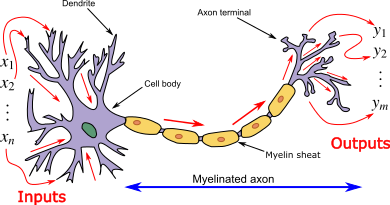
\includegraphics{neuron}
\centering
\caption{Neuron and mylinated axon with signal flow by Egm4313.s12 (Prof. Loc Vu-Quoc) - Own work, CC BY-SA 4.0, \url{https://commons.wikimedia.org/w/index.php?curid=72816083}}
\end{figure}

Neural networks are not new, and are quite closely related to the work of Gauss and Legendre~\cite{calin2020deep} on polynomial regression.
This linear approximator takes the weights of the neuron $w_i$ and multiplies them by the input $x_i$ and compares them with a threshold (or bias, as we will refer to it), $b$. 
So for our linear approximator neuron $L$, we have: $L(x) = \sum_{i=1}^{n}w_i x_i - b$.
In order to determine whether or not this neuron ``fires'', we use a nonlinear activation function such as the Heaviside function, the sigmoid function, or the rectified linear unit (ReLU), which we denote $\sigma$. 
We define the Rectified Linear Unit (ReLU) by $\sigma: \mathbb{R} \to \mathbb{R}$ 
$$\sigma(z) = max\{0, z\}$$
and so the output of our neuron is given by:
$$\hat{y} = \sigma\bigg(\sum_{i=0}^{n}w_i x_i\bigg)$$
where $w_0 = b$ and $x_0 = - 1$ to account for the bias term.

The weights are initialized randomly when the network is instantiated, and are updated during the training process.
In order to update the weights, a loss function must be specified.
This loss function will take the output of the neural network $\hat{y}$ and compare this prediction with the true value $y$ to assess the error.
Loss functions are too numerous to go through in detail here, so we refer interested readers to Goodfellow~\cite{goodfellow2016deep} for details.
For our purposes, we are interested in a classification task, and so we use the cross-entropy loss, defined as:
$$J = -\sum_{c=1}^{M} y_{o,c} \ln(\hat{y}_{o,c})$$
Where
$$y_{o,c} =
\begin{cases}
1 \quad\text{if class label $c$ is correct for observation $o$}\\
0 \quad\text{otherwise}	
\end{cases}
$$
and $\hat{y}_{o,c}$ is the predicted probability that observation $o$ belongs to class $c$
Since our number of classes, $M = 2$, this simplifies to:
$$J = -[y \ln(\hat{y}) + (1 - y) \ln(1 - \hat{y})]$$

In order to update our weights, we must take the gradient of the loss function, $\nabla J$, and then update the weights of each layer by backpropogation: 
$$w_t = w_{t-1} - \alpha * \nabla J_{t-1}$$
where $\alpha$ is the learning rate.
There are many optimization algorithms which can be used by neural networks and this is an active area of research.
Throughout our text, we use stochastic gradient descent~\cite{hastie01statisticallearning} without momentum.

Much of the power of neural networks as compared to standard polynomial regression stems from their incredible ability to generalize to previously unseen data.
Cybenko~\cite{cybenko1989approximation} first proved that 2-layer neural networks using sigmoid activation functions can uniformly approximate any continuous function of n real variables with support in the unit hypercube.
This result has been extended several times to other activation functions and networks of bounded width and depth. 
Due to Lu \textit{et al.}~\cite{lu2017expressive}, we can state the following:

\begin{theorem}
Let $f: \mathbb{R}^n \to \mathbb{R}$ be a Lebesgue-measurable function satisfying
$$\int_{\mathbb{R}^n} \abs{f(x)} dx < \infty$$
then for any Lebesgue-integrable function $f$ and $\epsilon \in \mathbb{R}; \epsilon > 0$, there exists a fully-connected ReLU network $\mathcal{A}$ of width $d_m \leq 4 + n$ such that the function $F_{\mathcal{A}}$ represented by the neural network satisfies:
$$\int_{\mathbb{R}^n} \abs{f(x) - F_{\mathcal{A}}(x)}dx < \epsilon$$
\end{theorem}

Despite the strength of these results, representation learning and neural network interpretability are open questions.
At present, little is understood about the exact mechanism by which neural networks are able to learn, and what the meaning of the learned representation is.
Some theories exist and since many of them are not mutually exclusive, it stands to reason that several may be true.
In particular, we will consider the information bottleneck theory~\cite{tishby2015deep, fischer2020conditional} from a geometric point of view.

\section{Prior Work}
Our work leverages an expanded dataset from Watkins \textit{et al.}~\cite{watkins2013using} and one of our objectives, as in Watkins's work, is to build a model which sufficiently detects Android malware using the interarrival time of Internet Control Message Protocol (ICMP) ping packets.
In the literature, decision trees were used to classify traffic.
Other work on the dataset by Watkins's team more closely mirrors our own, and details are elaborated in section~\ref{chap:three}.
In order to compare to Watkins's results to our own neural network results, we leverage a random forest from the Scikit-learn~\cite{scikit-learn} Python package to serve as a baseline.
Our work differs in that rather than seeking to optimize our ability to detect malware, we use this as a dataset with practical impact, for which we do not know the efficacy of neural networks.

The use of Fourier transforms in neural networks has been of interest for some time, and there are several papers on the subject~\cite{osowski2002fourier, pratt2017fcnn, highlander2016very} which consider these applications.
The choice to explore Fourier transforms in convolutional neural networks is natural, as the dot product is much faster than a convolution operation which relies on a sliding kernel. 
We lean most heavily on the paper by Pratt \textit{et al.}~\cite{pratt2017fcnn} due to its recency and implementation details. 
Particularly, Pratt considers the impact of the convolution theorem within neural networks and uses the Fast Fourier Transform to quickly compute $\mathcal{F}(\kappa * u) = \mathcal{F}(\kappa) \odot \mathcal{F}(u)$ where $\mathcal{F}$ is the Fast Fourier Transform, $*$ denotes convolution, and $\odot$ denotes the Hadamard pointwise Product.
They also describe a Fourier Pooling Layer to reduce the data size while retaining information by truncating the boundaries of the matrices.
Ultimately, the paper shows that on the CIFAR-10 and MNIST datasets, the overall accuracy is lower than benchmark results - though the network trains and evaluates images much more quickly.
Interestingly, we found the opposite results, which we detail in section~\ref{chap:three}.

Wavelet neural networks pioneered by Fujieda \textit{et al.}~\cite{fujieda2017wavelet} have shown promise for generalized pooling and convolution by abstracting them into downsampling and filtering in the spectral domain.
The results in the Fujieda paper were significant, as the network achieved better accuracy results than AlexNet on the target dataset while having approximately 1/4 the number of parameters.
In addition, the memory requirements and speed of the network were a significant improvement on the other architectures considered by Fujieda.
It is worth noting that implementation details from Fujieda are sparse, and so our implementation may differ from this reference implementation in some way, though the spirit and overall methods are the same.

Our work also considers and builds upon the Information Bottleneck theory of Neural Networks introduced by Tishby~\cite{tishby2015deep}.
The information bottleneck theory of deep learning suggests that the goal of supervised learning is to capture and efficiently represent the relevant information about the input data about the target data. 
In the process of creating a minimal sufficient statistic, a maximally compressed mapping of the input which minimizes mutual information is generated.
Tishby does this by demonstrating that the layered structure of the network creates a Markov chain of intermediate representations which forms the sufficient statistics.
The paper also suggests learning via information bottleneck, which we do not leverage.

Many of the issues with the information bottleneck theory are addressed in a controversial paper by Saxe~\cite{saxe2019information}.
Saxe argues compellingly that many of the issues with the saturation of nonlinearities such as tanh are not observed with ReLU.
Additionally, it argues - using empirical results - that networks which do not compress can still generalize. 
Saxe does not, however, argue that the fundamental conceit of the information bottleneck theory still holds and that an information theoretic approach to neural networks is still critical.

Fischer~\cite{fischer2020conditional} improves on Tishby's work by addressing Saxe's concerns and experimenting with both deterministic models as well as Variational Information Bottleneck~\cite{alemi2016deep} models. 
Fisher suggests that problems with robust generalization and lack of compression stem from models retaining too much information about the training data.
The Conditional Entropy Bottleneck model proposed by Fisher directly optimizes what he calls the Minimum Necessary Information criteria. 
Our work leans on the minimum necessary information criterion as a point of theory and we detail it in section \ref{chap:two}.

\section{Content of this Thesis}
Wavelet transforms and the Fourier transform were considered for use as powerful tools from signal processing which have wide-ranging uses and implications well beyond malware classification.
Our initial expectation was that these tools would serve to enhance the ability of networks to learn by extracting features from the raw data, processing it into a form which would give the neural network a more robust feature set to learn from.
During the experiments, the transformations seemed not to alter the ability of the network to learn, and we looked to information theory for an explanation. 
In our consideration of the network as a manifold and the weights of the network as projections of our data as a coordinate system on that manifold which is optimized through gradient descent, much of the literature discussed below gave us a theoretical framework on which to build understanding of our results. 
This work is presented in the following order, which allows the reader to understand the results through this framework, despite our malware dataset experiments being the motivation for the research.
\begin{itemize}
	\item In Chapter~\ref{chap:two}, we cover the necessary information theory to contextualize the results of this thesis. We cover common terminology, all of which is covered in greater depth in the canonical introduction to information theory by Cover and Thomas~\cite{coverthomas2006}. We move on to prove an important result about preservation of mutual information under homeomorphism. We introduce the information bottleneck and the concept of minimum necessary information,  which further contextualizes our results. We then discuss a geometric view of neural networks, and how the optimal weights of the neural network can be viewed geometrically as the orthonormal projection of the target onto the manifold of the neural network.
	\item In Chapter~\ref{chap:five}, we treat the MNIST dataset as our baseline for performance and introduce our methods which we use across our experiments on our malware dataset. We explain the four neural network architectures and three of the dataset transformation methodologies we use in our experiments. This experiment was conducted last, to confirm our findings from our experiments on the malware dataset, but is presented first to set the stage for our results. We choose MNIST as our baseline dataset; due to the vast amount of literature on MNIST, it has been referred to as the "Drosophila of machine learning"~\cite{goodfellow2016deep}, making it suitable to contextualize our results. We also capture the information plane representation of mutual information in the network similar to prior research~\cite{shwartz2017opening, saxe2019information}.
	\item In chapter~\ref{chap:three}, we address our malware problem and dataset. We conduct transforms on our data and treat the raw, Fourier, and Wavelet-transformed data as well as a dataset of summary statistics in line with Watkins~\cite{watkins2013using} with our two standard neural network models as well as two benchmark models which are introduced in chapter~\ref{chap:five}. We consider the mutual information as before, and address the accuracy results of the networks in question on our raw and summary datasets.
	\item In chapter~\ref{chap:four}, we consider Fourier and Wavelet neural networks inspired by prior work~\cite{pratt2017fcnn, fujieda2017wavelet} where the convolution theorem is exploited to learn representations. We again explore the information plane and potential advantages of using techniques which leverage the convolution theorem in-network.
	\item Finally, chapter~\ref{chap:conclusion} brings together the outcomes of our networks, baseline models, and information theoretic considerations of learning to explain our results. We consider avenues for further research and potential implications of our findings.
\end{itemize}
